\documentclass{beamer}
\usepackage[utf8]{inputenc}
\usepackage{graphicx}
\usetheme{Szeged}
\usecolortheme{wolverine}
\title{Probabilistic Dust Storm Prediction}
\subtitle{Presentation 2 -- Methodology}
\author{Sean Flaherty}
\date{2017}

\begin{document}
\frame{\titlepage}
\begin{frame}
	\frametitle{Overview}
	\begin{itemize}
		\item
			Goal: Use data mining/machine learning to create a predictive model for dust events on a local scale.
		\item
			Previous research: Univariate predictor (500mB geopotential height) using image processing (ZNCC). Only good at predicting large events [1]. 
		\item
			Justification: Want an accurate predictor for meso- and micro-scale dust events.
	\end{itemize}

\end{frame}
\begin{frame}
	\frametitle{Gathering Data}
	\begin{itemize}
		\item<-1->
			RAP/RUC forecast model -- NOMADS (NOAA Operational Model Archive and Distribution System).
		\item<-2-> Forecasts available from NOAA online repository (HTTPS/FTP).
		\item<-3-> Data downloaded using GNU wget utility [2].
	\end{itemize}
\end{frame}
\begin{frame}
	\frametitle{Data Format}
	\begin{itemize}
		\item
			GRIB -- GRIdded Binary (WMO standard for weather data).
		\item
			RAP/RUC models update forecasts hourly with 13 and 25.2 km resolutions.
		\ite
			Each file contains forecast models for a single time.
		\item
			Each file has a number of weather parameters, each of which with a grid of data points corresponding to locations.	
	\end{itemize}
\end{frame}

\begin{frame}
	\frametitle{GRIB Example}
	\centering
	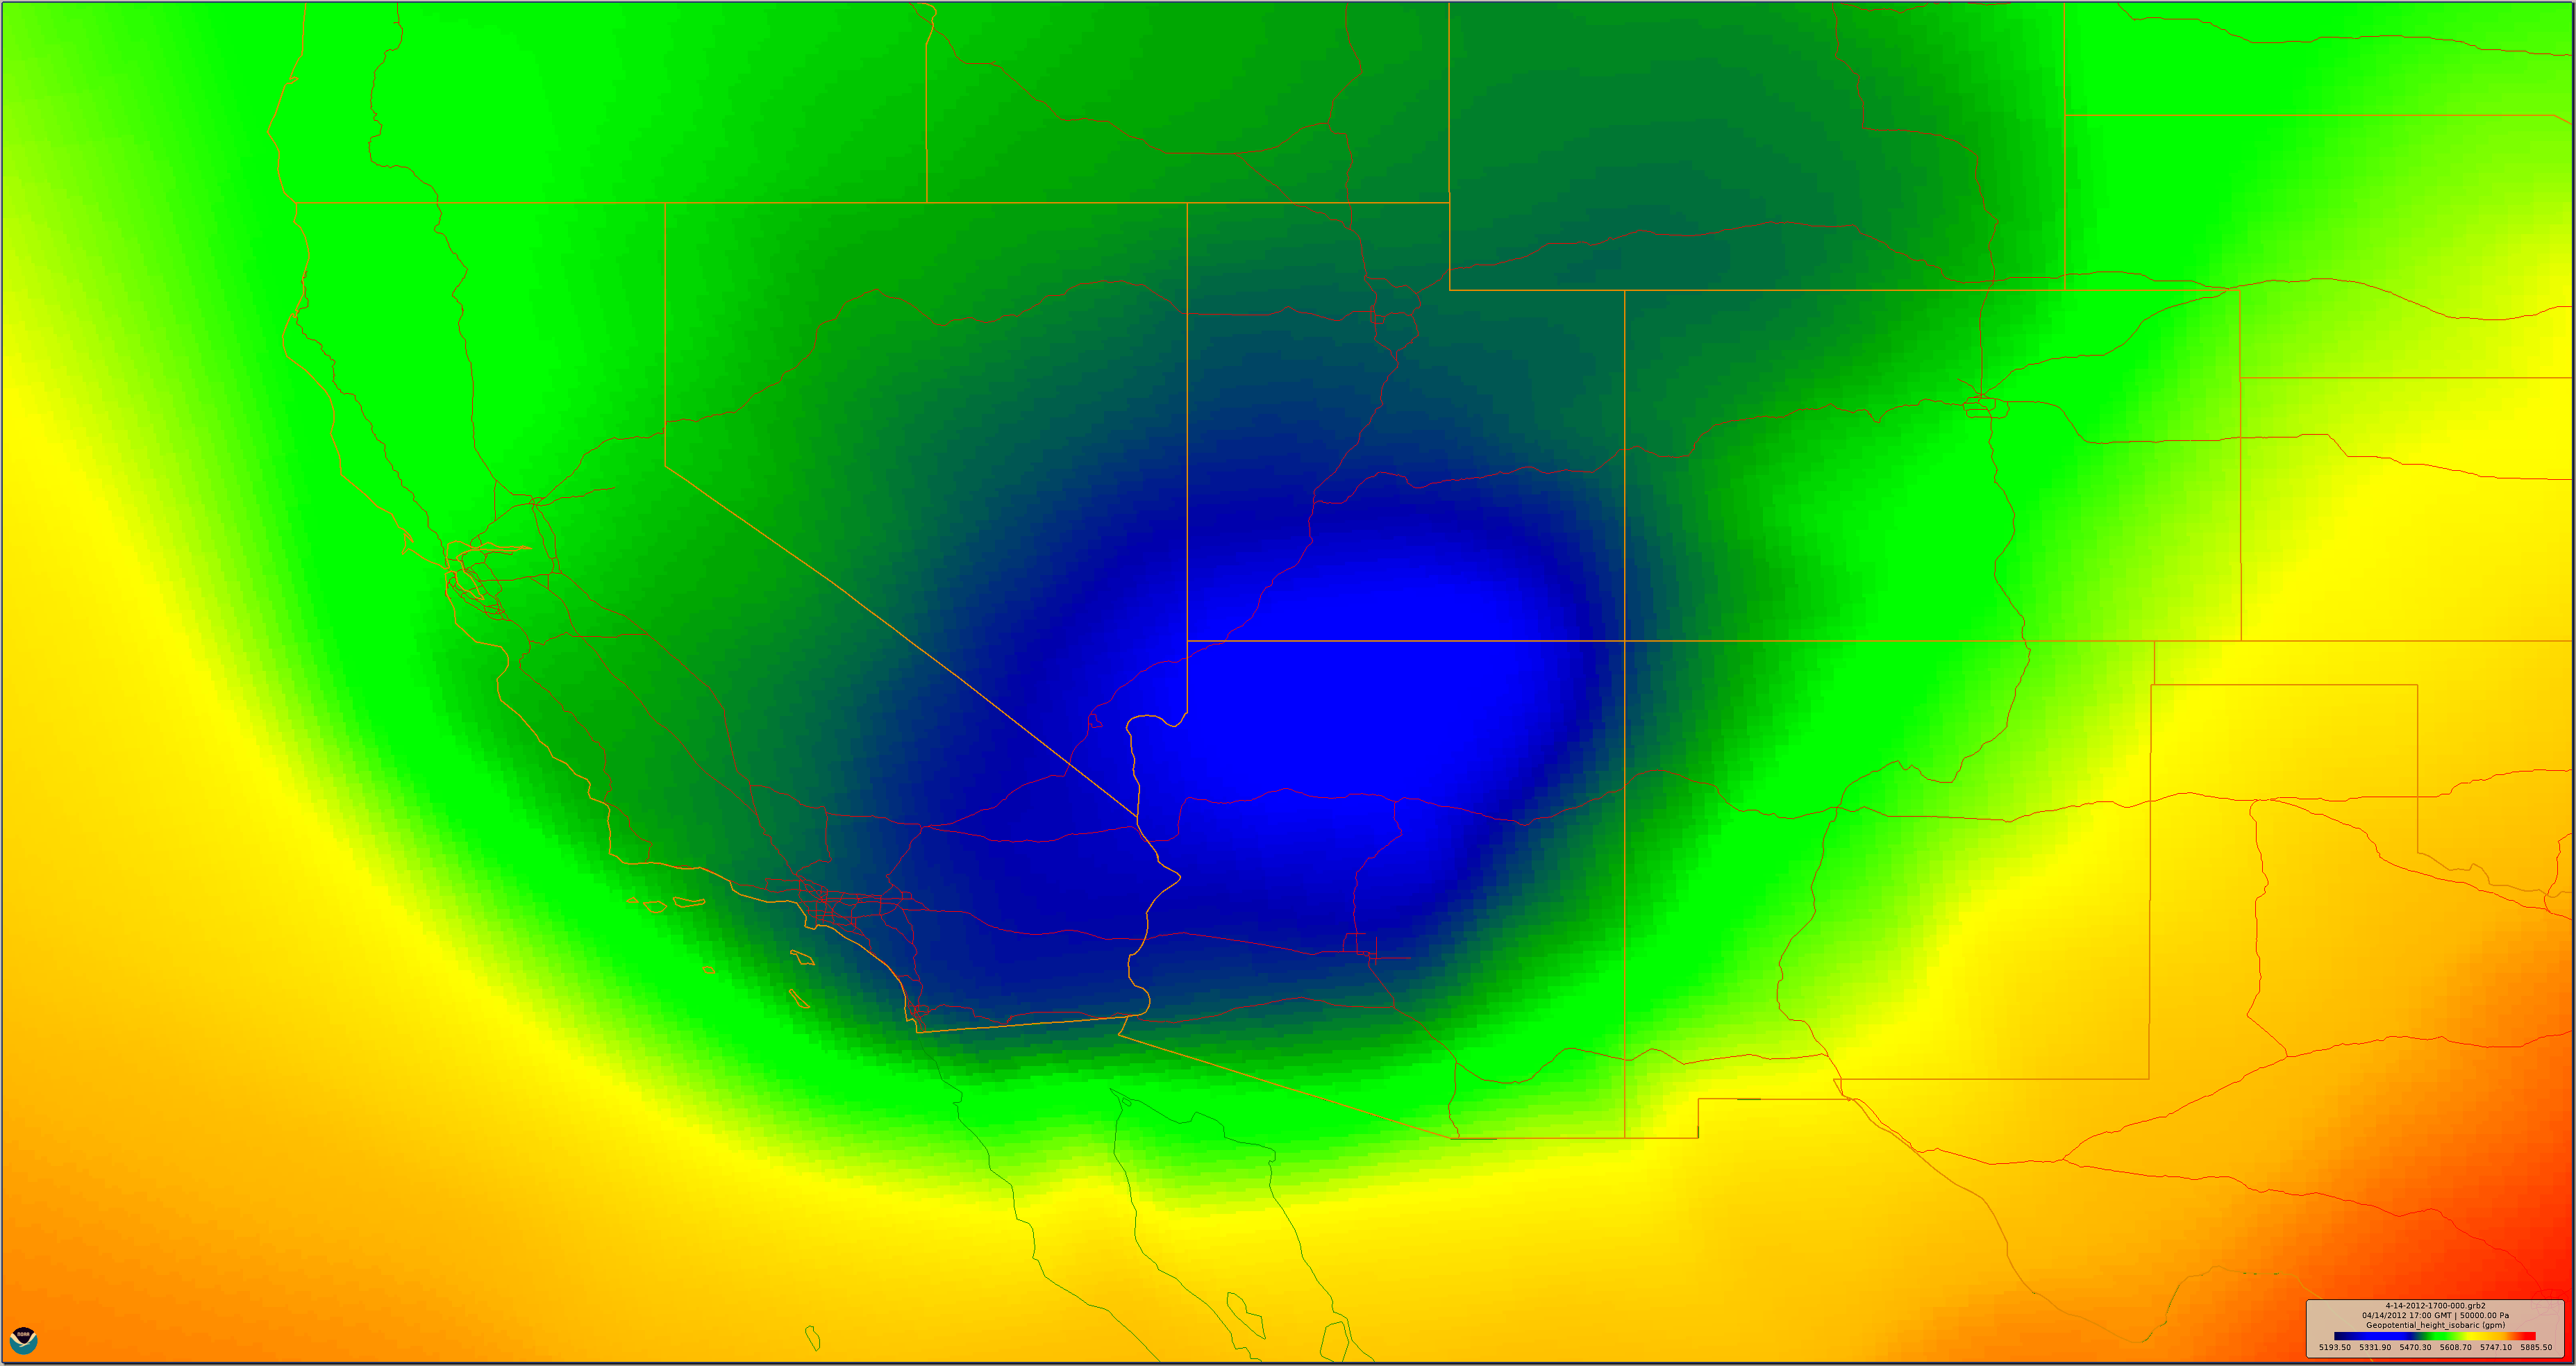
\includegraphics[width=0.75\textwidth]{images/abqlow.png}

	A single parameter's raster shown using NOAA Weather and Climate Tool. This image shows the 500mB geopotential height at 18:00GMT preceding a dust event on April 14, 2012 [3].


\end{frame}
\begin{frame}
	\frametitle{Reading GRIB files}
	\begin{itemize}
		\item
			pygrib Python library -- allows opening of .grb, .grb2 files in Python
		\item
			Opening a GRIB creates a file iterator, with each object in it a weather parameter [4].
		\item
			Each weather parameter has various attributes, including a raster of latitudes/longitudes and data for the parameter.
		\item
			Weather data gets stored into CSV files for easier lookup.
	\end{itemize}

\end{frame}
\begin{frame}
	\frametitle{PCA}
	\begin{itemize}
		\item
			Principal component analysis reduces the dimensionality of the data.
		\item 
			Transforms data into subspaces with the most spread between points - explains most of the variance in the data.
		\item
			RUC dataset has 315 dimensions for each instance -- could make algorithms less effective (curse of dimensionality).


	\end{itemize}

\end{frame}

\begin{frame}
	\frametitle{PCA plots}
	\begin{columns}
		\column{0.5\textwidth}
		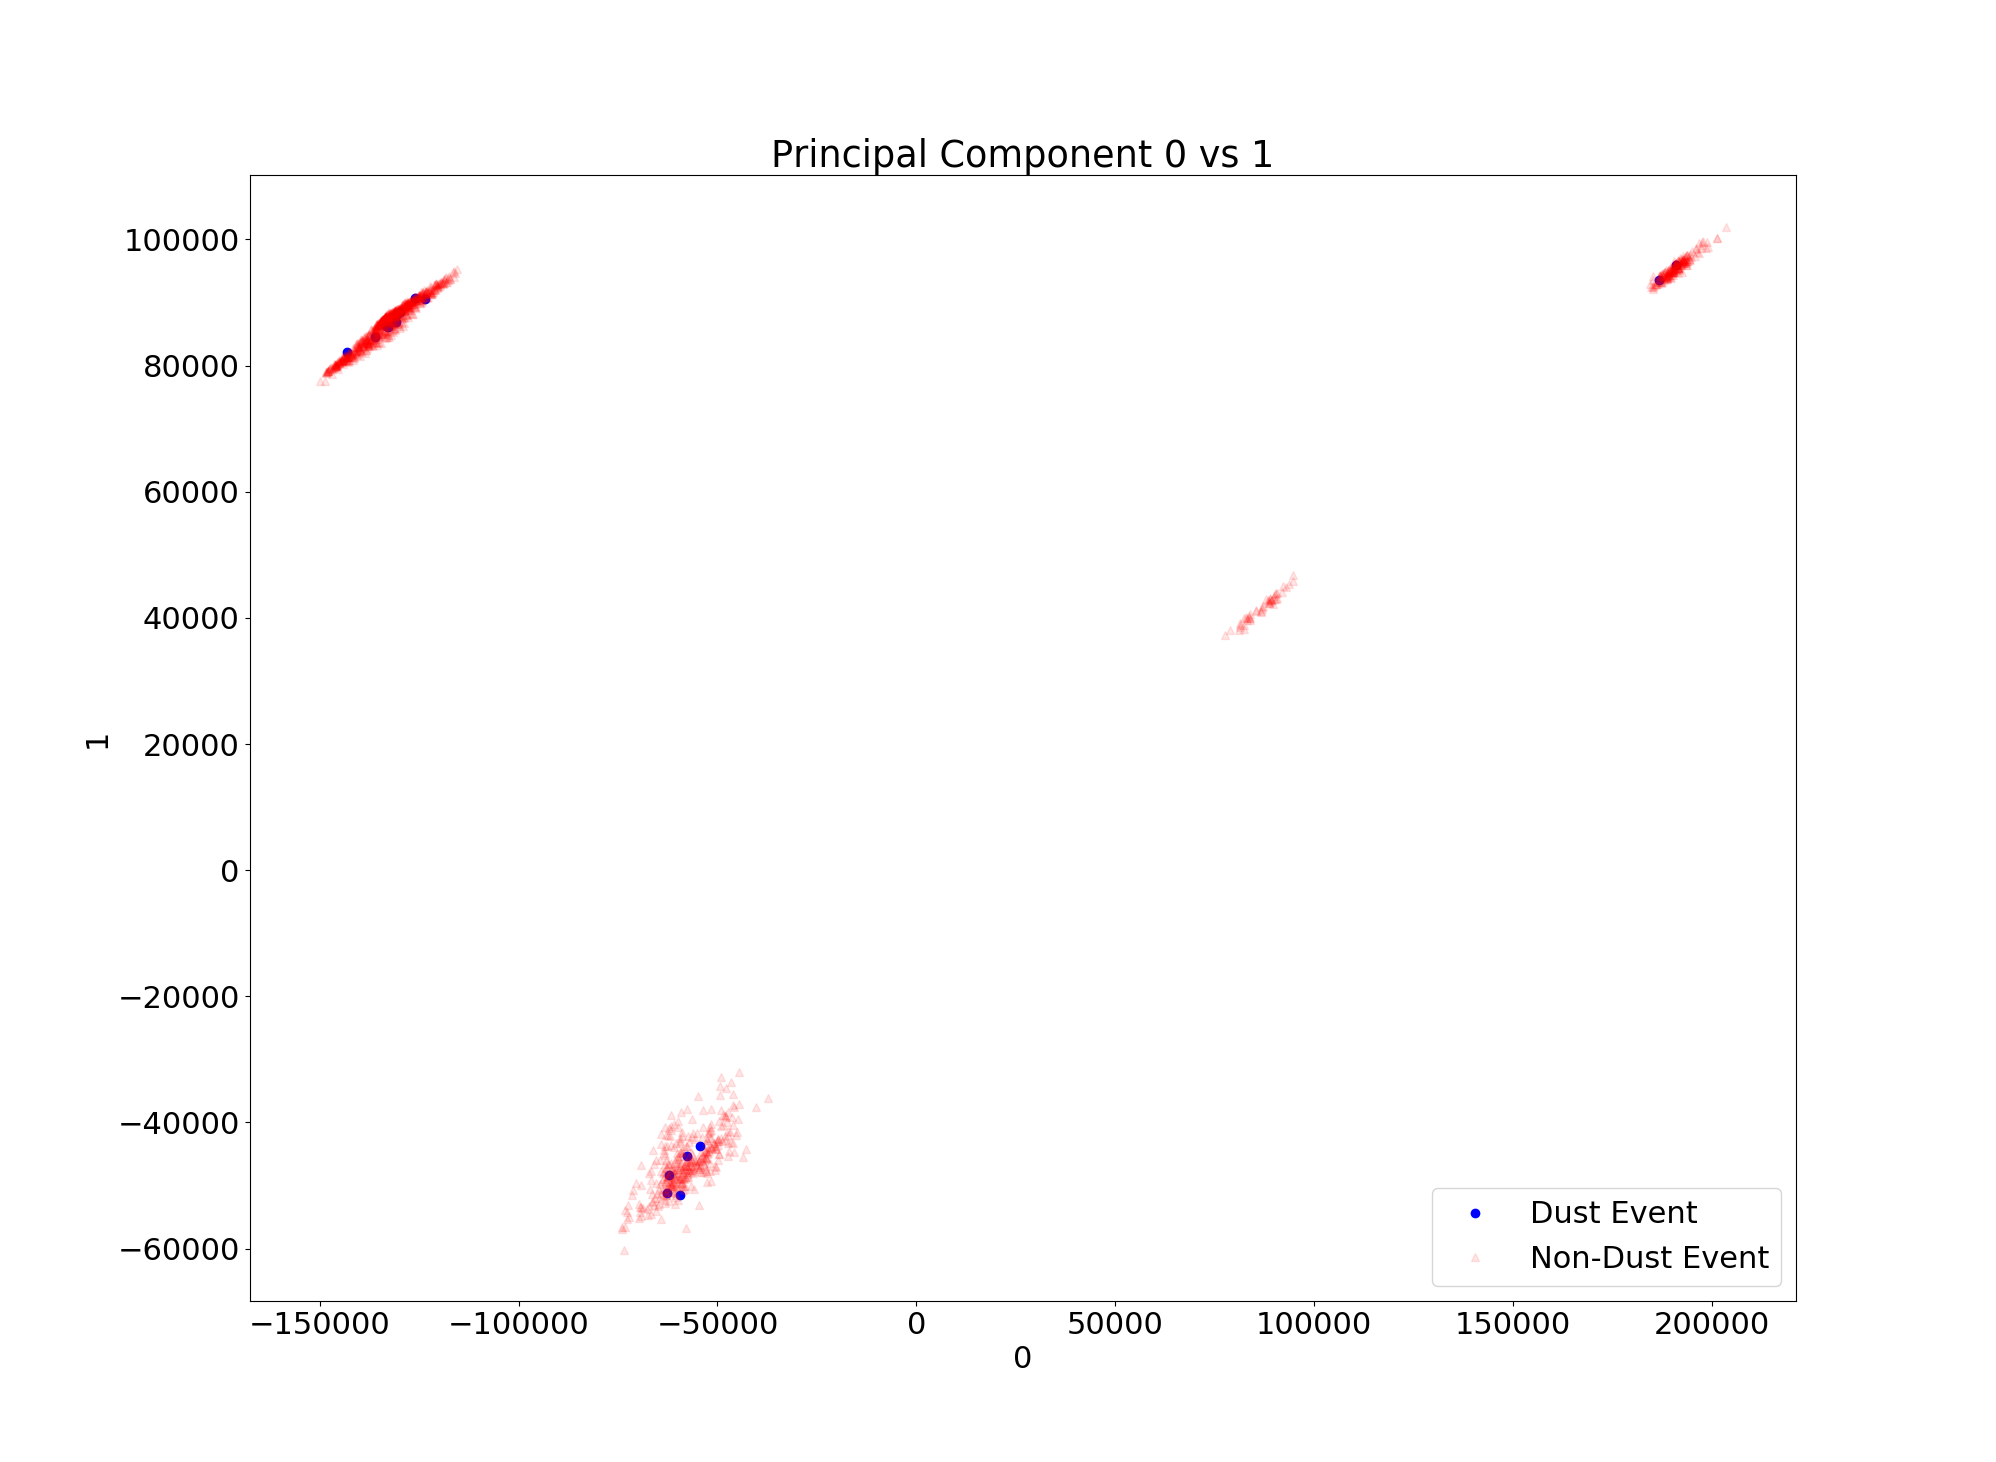
\includegraphics[width=\textwidth]{images/0vs1.png}
		\column{0.5\textwidth}
		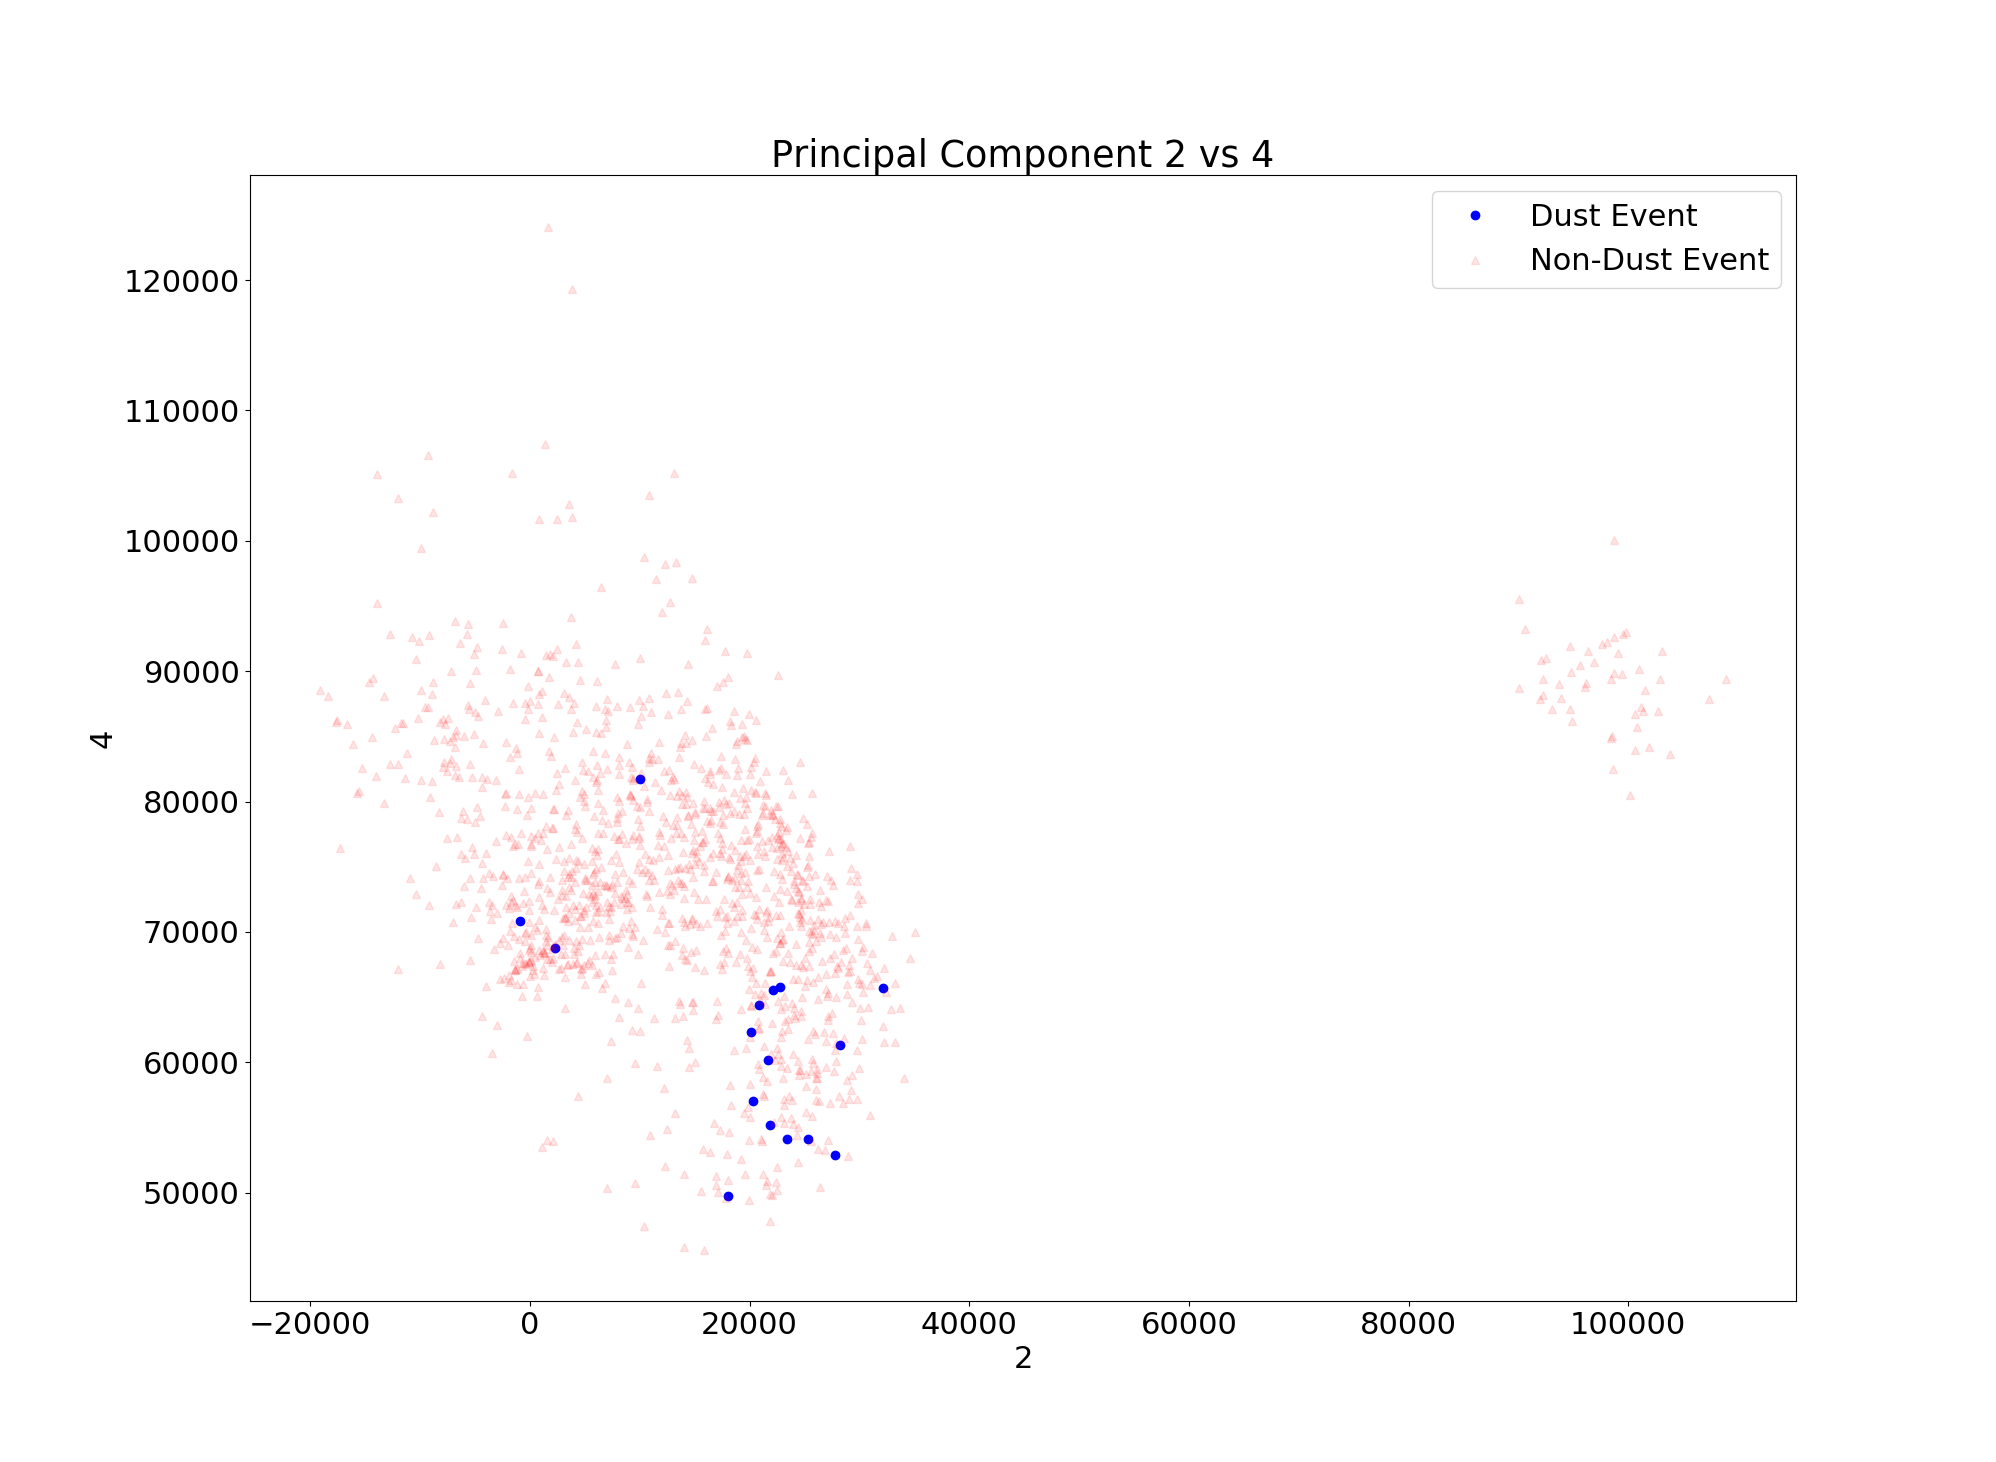
\includegraphics[width=\textwidth]{images/2vs4.png}
	\end{columns}

	Plots of principal components against each other. Left shows little no distinction between dust and non-dust events, while right shows some.
\end{frame}

\begin{frame}
	\frametitle{Algorithms}
	\begin{columns}
		\column{0.5\textwidth}
		\begin{itemize}
			\item
				Feedforward NN
			\item
				Feedforward NN with PCA
			\item
				RNN/LSTM
			\item
				RNN/LSTM with PCA
		\end{itemize}

		Try each algorithm and see which one provides the best accuracy.
		\column{0.5\textwidth}
		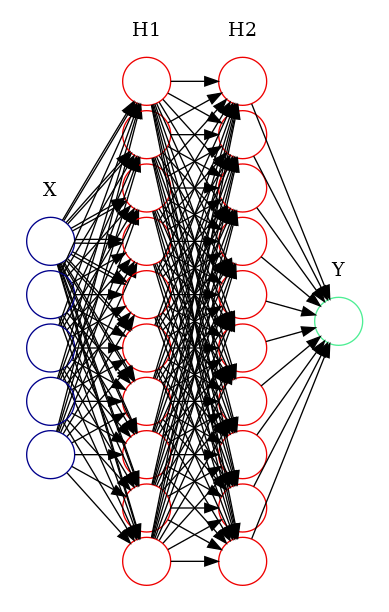
\includegraphics[width=0.75\textwidth]{images/nngraph.png}
	\end{columns}
\end{frame}
\begin{frame}
	\frametitle{Implementation of algorithms}
	\begin{columns}
		\column{0.5\textwidth}
		\begin{itemize}
			\item
				TensorFlow Python library
			\item
				Machine learning utility for creating computation graphs, doing lazy evaluations, using GPU for faster processing.
			\item
				Automates backpropagation and optimization algorithms [5].
		\end{itemize}
		\column{0.5\textwidth}
		
\includegraphics[width=\textwidth]{images/tensorflow.png}
	\end{columns}
\end{frame}

\begin{frame}
	\frametitle{References}
	[1] Armenta, Rebecca B. "Geopotential height patterns at 500mb associated with dust storms in the United States/Mexico border region during January-May of 2011-2014." May 2016 New Mexico State University.  Access May 31 2017.

	[2] "GNU Wget 1.18 Manual." GNU Project. Web. Jun. 27 2017.

	[3] "Rapid Refresh (RAP)." National Centers for Envrionmental Information. NOAA. Web. Jun. 27. 2017.

	[4] "pygrib documentation." Github. Dec. 29 2014. Web. Jun. 14 2017.

	[5] "Getting Started with TensorFlow." TensorFlow. Web. Jul. 5 2017.

\end{frame}
\end{document}
